\documentclass[]{article}

\usepackage[italian]{babel}
\usepackage[margin=20mm, footskip = 20pt]{geometry}
\usepackage{array}
\usepackage{tabularx}
\usepackage{graphicx}
\usepackage{subfiles}
\usepackage{hyperref}
\usepackage{nameref}
\usepackage{titlesec}
\usepackage{longtable}
\usepackage[table]{xcolor}
\usepackage{titling}
\usepackage{lastpage}
\usepackage{ifthen}
\usepackage{calc}
\usepackage{soulutf8}
\usepackage{contour}
\usepackage{float}
\usepackage{fancyhdr}
\usepackage{multirow}
\usepackage{pgfgantt}
\usepackage{lscape}

\newcommand{\hr}{\par\vspace{-.1\ht\strutbox}\noindent\hrulefill\par}

\graphicspath{ {./}
	{./commons/res}
}

%--------------------------------------------------
% Comandi per inserire contenuto del documento
%--------------------------------------------------
\makeatletter

\newcommand\appendToGraphicsPath[1]{%
	\g@addto@macro\Ginput@path{{#1}}%
}

\newcommand{\setTitle}[1]{%
	\newcommand{\@phTitle}{#1}%
}
\newcommand{\phTitle}{\@phTitle}

\newcommand{\setDate}[1]{%
	\newcommand{\@phDate}{#1}%
}
\newcommand{\phDate}{\@phDate}

\newcommand{\setUso}[1]{%
	\newcommand{\@uso}{#1}%
}
\newcommand{\uso}{\@uso}

\newcommand{\setVersione}[1]{%
	\newcommand{\@versione}{#1}%
}
\newcommand{\versione}{\@versione}

\newcommand{\disabilitaVersione}{%
	\renewcommand{\setVersione}[1]{}%
	\renewcommand{\versione}{DISABILITATA}
}

\newcommand{\setResponsabile}[1]{%
	\newcommand{\@responsabile}{#1}%
}
\newcommand{\responsabile}{\@responsabile}

\newcommand{\setRedattori}[1]{%
	\newcommand{\@redattori}{#1}%
}
\newcommand{\redattori}{\@redattori}

\newcommand{\setVerificatori}[1]{%
	\newcommand{\@verificatori}{#1}%
}
\newcommand{\verificatori}{\@verificatori}

\newcommand{\setModifiche}[1]{%
	\newcommand{\@modifiche}{#1}%
}
\newcommand{\modifiche}{\@modifiche}

\makeatother 

%--------------------------------------------------
% Comandi per i documenti esterni e il glossario
%--------------------------------------------------

\newcommand{\dext}[1]{\textsc{#1\textsubscript{\textit{D}}}}

\newcommand{\glock}[1]{\textsc{#1\textsubscript{\textit{G}}}}

%--------------------------------------------------
% Comandi per impostare sottotitoli di quarto e quinto livello
%--------------------------------------------------

\setcounter{secnumdepth}{4}
\setcounter{tocdepth}{4}

\titleformat{\paragraph}
{\normalfont\normalsize\bfseries}{\theparagraph}{1em}{}
\titlespacing*{\paragraph}{0pt}{2.25ex plus 1ex minus .2ex}{1.5ex plus .2ex}

\titleformat{\subparagraph}
{\normalfont\normalsize\bfseries}{\thesubparagraph}{1em}{}
\titlespacing*{\subparagraph}{0pt}{1.75ex plus 1ex minus .2ex}{.75ex plus .1ex}

\appendToGraphicsPath{../../../commons/res/}

%------------------------------
%
% COMANDI DI CONFIGURAZIONE
%
%------------------------------

\setTitle{Verbale riunione \#30}

\setVersione{0.1.0}

\setDate{01-04-2021}

\setResponsabile{Paolo Scanferlato}

\setRedattori{Alessandro Dindinelli}

\setVerificatori{Lucia Fenu}

\setUso{Interno}

\setModifiche{
	0.1.0 & Lucia Fenu & Verificatore & 01-04-2021 & Verifica della prima stesura\\
	0.0.0 & Alessandro Dindinelli & Amministratore & 29-03-2021 & Prima stesura}

\begin{document}

	% Direttive per la creazione del titolo tramite comando maketitle
\title{\huge \textsc{\phTitle{}} \\
	\vspace{11pt} \large \textsc{\phDate{}}}

\author{} % Non toccare
\date{} % Non toccare

%--------------------
% Frontespizio
%--------------------

% Logo del gruppo
\begin{figure}[t!]
	\centering
	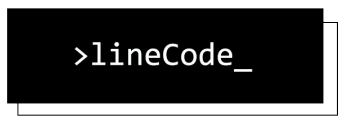
\includegraphics[width=20em]{lclong}
\end{figure}

% Titolo / Nome
\maketitle
\thispagestyle{empty}

% Dati specifici sul doc in forma tabulare
\begin{table}[ht]
	\begin{center}
		\label{tab:Dati sul documento}
		\begin{tabular}{r|l}
			\multicolumn{2}{c}{ \textsc{Dati sul documento} } \\
			\hline
			\textbf{Versione} & \versione{} \\
			\textbf{Uso} & \uso{}  \\
			\textbf{Redattori} & \redattori{} \\
			\textbf{Verificatori} & \verificatori{} \\
			\textbf{Responsabile} & \responsabile{} \\
			\textbf{Destinatari} & lineCode \\
								& prof.\ Vardanega Tullio \\		
								& prof.\ Cardin Riccardo \\
			\ifthenelse{\equal{\uso}{Esterno}}{
								& Sanmarco Informatica
			}{} \\
		\end{tabular}
	\end{center}
\end{table}

\newpage

\renewcommand{\arraystretch}{2} % allarga le righe con dello spazio sotto e sopra
\begin{longtable}[H]{>{\centering\bfseries}m{2cm} >{\centering}m{3.5cm} >{\centering}m{2.5cm} >{\centering}m{3cm} >{\centering\arraybackslash}m{5cm}}
	\rowcolor{lightgray}
	{\textbf{Versione}} & {\textbf{Nominativo}} & {\textbf{Ruolo}} & {\textbf{Data}} & {\textbf{Descrizione}}  \\
	\endfirsthead%
	\rowcolor{lightgray}
	{\textbf{Versione}} & {\textbf{Nominativo}}  & {\textbf{Ruolo}} & {\textbf{Data}} & {\textbf{Descrizione}}  \\
	\endhead%
	\modifiche{}%
\end{longtable}

	\newpage

	%--------------------------------
	%
	% IL CONTENUTO INIZIA DA QUI
	%
	%--------------------------------

		\section{Introduzione}
		\subsection{Luogo e data dell'incontro}
		\begin{itemize}
			\item \textbf{Modalità}: Telematica;
			\item \textbf{Software utilizzato}: \glock{Discord};
			\item \textbf{Data}: 29 Marzo 2021;
			\item \textbf{Ora di inizio}: 16:00;
			\item \textbf{Ora di fine}: 19:30.
		\end{itemize}

		\subsection{Presenze}
		\begin{itemize}
			\item \textbf{Presenti}:
			\begin{itemize}
				\item Matteo Alba
				\item Giacomo Bulbarelli
				\item Alessandro Chimetto
				\item Alessandro Dindinelli
				\item Lucia Fenu
				\item Paolo Scanferlato
				\item Valton Tahiraj
			\end{itemize}
			\item \textbf{Assenti}:
			\begin{itemize}
				\item Nessuno
			\end{itemize}
		\end{itemize}


		\subsection{Ordine del giorno}
		\begin{enumerate}
			\item Coordinamento lavori sistema di comunicazione;
			\item revisione correzione documenti RP;
			\item suddivisione lavori.
		\end{enumerate}

	\newpage

	\section{Svolgimento}
		\subsection{Coordinamento lavori sistema di comunicazione}
		Ci si è sincronizzati sullo stato dei lavori riguardo il cambio tecnologico tra \glock{API Rest} ed \glock{Atmosphere}, per il miglioramento del sistema di comunicazione tra le sue componenti. \\
		I lavori proseguono bene ma non sono completati, e richiederanno ancora del lavoro.
		\\
		
		\subsection{Revisione correzione documenti RP}
		Si è letto insieme la correzione dei documenti consegnati in RP, pubblicata dal Prof. Vardanega. Sono stati discussi tutti i punti riscontrati, ragionando sulle motivazioni per le quali tali errori si siano verificati e decidendo quali siano le giuste correzioni da apportare. \\
		Essendo sorti dei dubbi riguardo delle particolari correzioni, si è deciso di scrivere una mail ai rispettivi professori per richiedere dei chiarimenti a riguardo.
		Si è provveduto a fissare un incontro con il referente di Sanmarco Informatica, per discutere delle metodologie per verificare i requisiti prestazionali ed altre eventuali problematiche riscontrate.
		\\
		
		\subsection{Suddivisione lavori}
		Ci si organizzati per il proseguimento dei lavori, decidendo di dividersi in due gruppi: uno che prosegua i lavori di miglioramento al sistema di comunicazione, e l'altro che inizi la produzione degli schemi dell'architettura del sistema, fino alla successiva riunione del gruppo.
		\\


	\subsection{Riunione successiva}
	Riunione successiva fissata in:
	\begin{itemize}
		\item \textbf{Data}: 31-03-2021;
		\item \textbf{Ora}: 10:00;
		\item \textbf{Modalità}: Telematica: \glock{Google Meet}.
	\end{itemize}

	\newpage

	\section{Tabella delle decisioni}

	\begin{table} [h!]
		\rowcolors{2}{gray!25}{gray!6}
		\begin{center}
			\begin{tabular} { m{2cm} m{14cm} }
				\rowcolor{lightgray}
				\textbf{ID} & \textbf{Decisione}\\
				V31.1 & I due gruppi di lavoro sono stati così divisi:
				 \begin{itemize}
					\item implementazione \glock{WebSocket}: Giacomo Bulbarelli, Alessandro Chimetto, Valton Tahiraj;
					\item architettura UI: Matteo Alba, Alessandro Dindinelli, Lucia Fenu, Paolo Scanferlato.
				\end{itemize}\\
				V31.2 & Migliorare l'attualizzazione dei rischi e popolarla maggiormente, ragionando su cosa è successo, perché è successo, e come ciò è stato affrontato. \\
				V31.3 & Migliorare la pianificazione, valorizzando gli incrementi, in base alle previsioni fatte in RR. \\
				V31.4 & Ricalcolo del consuntivo di periodo, e correzione, mantenendolo inferiore a quanto approvato in RR. \\
				V31.5 & Correggere il metodo di versionamento dei documenti in base a quanto verrà comunicato dal Prof. Vardanega. \\
				V31.6 & Correggere i casi d'uso in base alle correzioni espresse dal Prof. Cardin. \\
				V31.7 & Aggiungere requisito di qualità per la redazione del manuale utente. \\
				V31.8 & Spostare il requisito RMP2 nei requisiti di qualità. \\
				V31.9 & Verificare che nel PdQ i titoli delle sezioni rispettino le norme prefissate. \\
			\end{tabular}
		\end{center}
	\end{table}

\end{document}

